% ===========================================================================
\section{Validation}
\label{sec:validation}
% ===========================================================================

\subsection{Pakistan's own UNFCCC filing, cell-audited}
\label{sec:crt}

Pakistan filed Common Reporting Tables with the UNFCCC in 2024, for inventory year 2022. They
are the official statement of what the country reports for this category, and every figure
below is re-derived from the workbook's cells on each run, with the filing's arithmetic
(activity $\times$ implied factor $=$ reported emissions) reproduced exactly before anything
is compared.

The filing reports 1.A.1.a at \SI{777243}{} TJ and \SI{62841}{\kilo\tonne} \COtwo{} for
calendar 2022, and three of its cells matter more than its total.

\textbf{The basis column reads NCV.} Every 1.A.1.a row states the net calorific basis---the
official answer to what Section~\ref{sec:heatrate} approached physically. The sector's largest
declared risk is now covered from two independent directions: the plant meters imply an
efficiency only a net basis supports, and the country's own filing states the basis outright.

\textbf{Gaseous fuels are not estimated.} The official public-electricity category carries NE
for gas, in a country whose regulator reports gas and RLNG as \SI{58}{\percent} of thermal
fuel energy---\SI{306000}{} TJ in this inventory's matched year with no official counterpart.
The filing's liquid-fuel activity is several times the regulator's fuel oil and diesel
combined, so a reallocation may be at work, but as filed the category either omits nearly half
the fleet's fuel or books it unlabelled. This is the kind of finding a cell-level official
comparison exists to surface, and no model comparator could have.

\textbf{The solid-fuel line corroborates two numbers here.} The CRT's \SI{324724}{} TJ agrees
with the regulator's coal energy to \SI{2}{\percent}---two institutions, one answer, which
cuts against the reading of the coal-NCV diagnostic in which the regulator's coal energy is
overstated by most of a factor of two. Section~\ref{sec:impliedcv} now sets a third channel
against both: the per-plant heat rates side with the diagnostic, leaving this agreement as
the counter-evidence rather than the settlement. And its implied \COtwo{} factor of \SI{97.57}{} t/TJ
sits at a \SI{46}{\percent} lignite share on IPCC endpoints: between this paper's superseded
\SI{35}{\percent} and its ledger-derived \SI{79}{\percent}, from 2022 when the Thar fleet was
mid-ramp---consistent with a fleet in transition.

The years overlap by half (calendar 2022 against July 2022--June 2023), so magnitude
comparisons bound rather than test; the fuel-scope and basis findings above do not depend on
the year at all.

\subsection{Grid generation against EDGAR}

EDGAR reports Pakistani power industry emissions at \SI{56.80}{\mega\tonne} \COe{} for 2024
\citep{edgar2025booklet}. This inventory reports the family reference
\SI{40.04}{\mega\tonne} (alternatives 38.45 heat-rate, 44.05 with K-Electric, 57.82 legacy
control) for FY2023--24, or \SI{70}{\percent} of it---different years, so the comparison
bounds rather than tests. That ratio was close to unity on the legacy control and the
direction of the change is not evidence either way:
EDGAR's power figure for Pakistan is built from the same international energy balances that
feed the aggregate fuel control this inventory stopped booking.

EDGAR remains the external benchmark; the official comparison above is the primary one. The taxonomy match is close:
EDGAR's power industry category is essentially 1A1a, built from the same kind of national fuel
statistics, so the comparison is nearly like-for-like rather than approximately so. Agreement
at \SI{142}{\percent} between two independently constructed estimates, in different reference
years, is about as close as this class of comparison gets.

The residual is plausibly captive and industrial self-generation, which NEPRA's scope excludes
and which EDGAR's power category may partly include. That reading is testable now in a way it
was not before: this inventory's captive category is \SI{5.55}{\mega\tonne}, so if EDGAR's
figure included all captive gas generation the two would be further apart, not closer. The
more likely reading is that EDGAR includes some self-generation and this inventory's grid
figure and EDGAR's differ by less than either's uncertainty.

\subsection{Captive gas self-generation against EDGAR's industrial combustion}

EDGAR reports Pakistani industrial combustion at \SI{43.98}{\mega\tonne}. This inventory
reports \SI{5.55}{\mega\tonne} against it, a ratio of \num{0.13}.

That ratio measures \emph{coverage}, not agreement, and the distinction matters enough that
the benchmark row says so explicitly. This category estimates one fuel in one use: gas burned
by industrial plants generating their own electricity. It does not estimate industrial process
heat, boilers, kilns, captive plants burning oil or coal or bagasse, or the kiln fuel behind
the cement category. A ratio near \num{0.13} is therefore the expected result rather than a
discrepancy to investigate, and a ratio near \num{1.0} would indicate an error.

The internal reconciliation is the one that has teeth. The plant register sums to
\SI{288.01}{} MMCFD against OGRA's independently published \SI{288}{}---two sources built from
different records agreeing to \SI{0.01}{}. That is what establishes the category is describing
Pakistan's captive fleet rather than a subset or a superset of it.

\subsection{The time series as an internal check}

\begin{figure}[htbp]
\centering
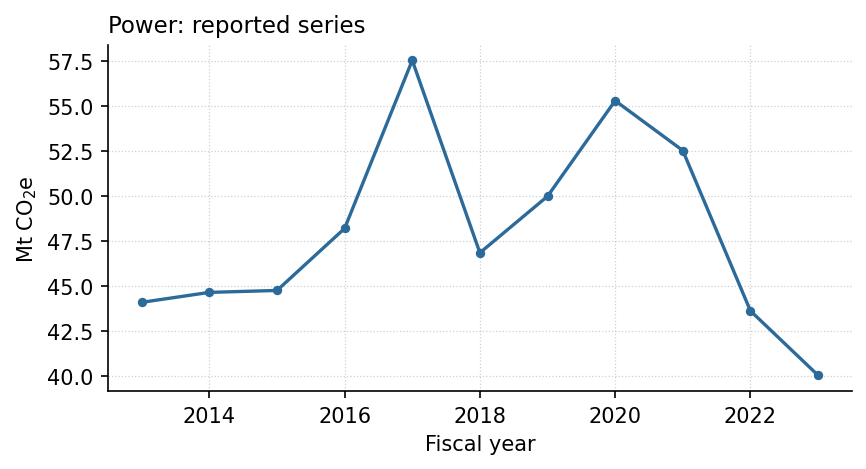
\includegraphics[width=\linewidth]{power_timeseries.png}
\caption{Grid emissions FY2013--24. The furnace-oil era's climb, its one-year collapse in
FY2018--19, the coal-era rise to FY2021--22 and the partial recovery track the fleet's own
history; the added early years parse from five earlier report editions, each reconciled
against its own printed totals.}
\label{fig:series}
\end{figure}

The series now runs eleven years, FY2013--14 to FY2023--24: \SI{44.09}{}, \SI{44.64}{},
\SI{44.75}{}, \SI{48.19}{}, \SI{57.52}{}, \SI{46.84}{}, \SI{49.98}{}, \SI{55.28}{},
\SI{52.51}{}, \SI{43.62}{} and \SI{40.04}{\mega\tonne} (the family reference; alternatives of three kinds: 38.45 heat-rate, a fuel-property alternative; 44.05 with K-Electric, a coverage alternative; 57.82 legacy control, the previously published account)---extended backward in this
revision by parsing five earlier report editions, every added year reconciling against its
edition's own printed Total row, with overlapping years reproduced identically across
editions. The shape is a fleet history: a climb through the furnace-oil era to the
FY2017--18 peak, a \SI{10.7}{\mega\tonne} fall in one year as oil retired, and the coal-era
climb to the FY2021--22 peak. Movements that large correspond to known fleet and demand
events rather than to smooth interpolation, which is what a series built from a modelled
activity proxy would produce.

What those movements were is now decomposed rather than narrated. An additive LMDI-I
decomposition over the fuel table---exact by construction, its terms closing to machine
precision---attributes the \SI{-4.1}{\mega\tonne} change from FY2013--14 to FY2023--24 as
\SI{-5.2}{\mega\tonne} of activity (less fuel energy booked), \SI{0.9}{\mega\tonne} of
mix and \SI{0.2}{\mega\tonne} of factor---and the mix term is close to a pure fuel swap:
coal contributes \SI{+21.0}{\mega\tonne} and furnace oil \SI{-24.2}{}, with gas at
\SI{+4.8}{}. A decade of Pakistani power-sector change is, in megatonnes, one fuel
replacing another.

\textbf{The direction of the total changed with the coal re-base, and the reason is the
activity term.} While the sector booked NEPRA Table 3's coal energy this decade read as a
rise, and this paragraph described the activity term as \emph{more} fuel energy burned.
Booking the generating stations' own metered coal at default rank calorific values instead
lowers the reference year's coal energy by \SI{46}{\percent} and FY2013--14's by only
\SI{36}{\percent}, so the booked total energy falls across the decade where the printed
conversion had it growing. The fuel swap is unaffected---it is a share, not a level---and
the coal and furnace-oil mix terms are what they were. What moved is the level, which was
the part Table 3's flat conversion was setting.
The one year the story is not mix is FY2021--22, whose \SI{-2.8}{\mega\tonne} step was
mostly activity (\SI{-3.2}{}): a demand story rather than a fleet change, in either
direction and on either coal account. The factor term is no
longer zero. An earlier edition applied the FY2023--24 coal blend to every year, so the
term vanished by construction, and this paragraph recorded that as a limitation and
predicted the true series would carry a small positive factor term as the fleet moved from
imported bituminous toward Thar lignite. The per-year blend is wired now---held in
\texttt{data/power\_coal\_blend\_by\_year.csv}, zero before the Thar fleet existed and
\num{0.79} at the reference year---and the prediction held at \SI{+0.2}{\mega\tonne}. The decomposition stays
inside Table~3 deliberately; folding in the generation table would import the coal
coverage mismatch of Section~\ref{sec:heatrate} and narrate an artefact as efficiency.

\subsection{The implied heat rate, and what it says about the activity tables}
\label{sec:heatrate}

The regulator's report contains two tables this inventory had never made talk to each other.
Table~3 gives fuel consumed by fuel; Table~17 gives net generation by fuel and system. Dividing
one by the other gives an implied heat rate---and a heat rate has physical bounds, so the ratio
tests whether the two tables describe the same fleet.

\begin{table}[htbp]
\centering
\footnotesize
\begin{tabular}{@{}lrrl@{}}
\toprule
\textbf{Fuel} & \textbf{Implied efficiency} & \textbf{Spread} & \textbf{Verdict} \\
\midrule
Gas (incl.\ RLNG) & \SIrange{37.7}{56.0}{\percent} & $\times$1.49 & stable \\
Furnace oil       & \SIrange{39.7}{52.1}{\percent} & $\times$1.31 & stable \\
Coal              & \SIrange{34.6}{39.3}{\percent} & $\times$1.14 & unstable \\
Diesel oil        & \SIrange{44.1}{50.2}{\percent} & $\times$1.14 & stable \\
\bottomrule
\end{tabular}
\caption{Implied net efficiency over the nine fiscal years both tables now cover,
FY2015--24, on material years (above \SI{1000}{GWh}).}
\label{tab:heatrate}
\end{table}

Gas is the reassuring row, and the longer window makes it more so, not less. Its implied
efficiency steps from \SIrange{38}{40}{\percent} in FY2015--17 to \SIrange{48}{56}{\percent}
from FY2018 onward---exactly when the RLNG combined-cycle fleet entered service---and then
holds. A ratio of two statistical tables that tracks a known fleet transition and then sits
stably at what combined cycles achieve on a net basis is behaving like real fuel energy
over real generation, in both eras.

Coal is not, on the account this check refuted. Read against NEPRA Table 3's published
coal energy its implied efficiency runs \SI{58.4}{\percent} in FY2020---above any coal plant
ever built, ultra-supercritical included---and \SI{34.6}{\percent} in FY2023--24, a three-fold
swing in four years. No fleet changes efficiency like that. The conclusion is that
Table~3's coal row and Table~17's coal row do not cover the same set of plants, and that the
mismatch moves between years.

Two things follow, and the second matters more than the first.

\textbf{This does not affect the emissions estimate.} The sector is driven by Table~3 alone.
The coverage of Table~17 is irrelevant to Equation~(1), and no number reported in this paper
changes because of the finding. It is published because a reader comparing this inventory's
implied generation against NEPRA's would otherwise discover the discrepancy unaided and have no
way to tell which table this sector used.

\textbf{It partly settles the sector's largest declared risk.} Section~\ref{sec:limitations}
records that the TOE figures may be on a gross rather than net calorific basis, worth
\SIrange{5}{10}{\percent} on \COtwo{}. Gas at a stable \SI{49}{\percent} net is what a combined
cycle does on a \emph{net} basis; read as gross, the same fuel would imply about
\SI{55}{\percent}, which is at the very top of what any fleet average reaches. That is evidence
for the net reading rather than proof of it. The risk stays declared---but it is no longer
untested, which it was for as long as this check went unrun.

The comparison rests on one mapping worth stating. Table~3 has a single ``Gas'' row while
Table~17 splits gas from regasified LNG, and the fuel table has no RLNG row at all---so the
fuel behind Table~17's RLNG generation can only sit inside Table~3's gas figure, there being
nowhere else in the table for it to be. A test asserts that no RLNG fuel row has appeared,
because if a future edition adds one, the mapping would double-count instead.

\subsection{Per-plant heat rates arbitrate the coal conversion}
\label{sec:impliedcv}

The heat-rate instability above asked for the plant-level tables, and the report carries
them: Tables~20, 23 and~28 publish per-plant heat rates in Btu/kWh for five fiscal years,
never previously parsed here. Table~28's footnote states the basis---LHV---so heat rate
times net generation is net-calorific fuel energy, and that energy over the ledger's coal
mass is a calorific value, plant by plant, with Table~3 nowhere in the loop.

Before trusting the channel, the gas plants test it, because for MMBTU-metered plants the
ledger holds true fuel energy. Three behaviours emerge, all reported: three plants (Liberty
Daharki, Sindh Nooriabad-I and -II) print net heat rates that reproduce the ledger's
fuel-over-generation ratio to four digits---fully circular, the heat rate \emph{is} the fuel
table; the pipeline-gas plants Uch and Uch-II sit at \numrange{1.104}{1.109} against the
net-export heat rate, exactly the natural-gas HHV/LHV factor, so same meters converted to
the LHV basis the footnote promises; and the RLNG combined cycles drift year to year, an
independent channel. No coal plant is in the circular set: six of eight print year-varying
operational heat rates, and Sahiwal and Thar Coal Block-I print flat design values (the
latter with a net heat rate below gross, which no plant can do; the cells are kept as
printed and flagged).

The result arbitrates the diagnostic. The Thar mine-mouth plants imply
\SIrange{10.7}{13.9}{} TJ/Gg across their plant-years, mass-weighted \SI{11.1}{} in
FY2023--24---squarely the IPCC lignite value of \SI{11.9}{}---and the imported-coal plants
\SIrange{19.1}{25.1}{}, the bituminous band. The FY2023--24 fleet, mass-weighted at
\SI{99}{\percent} ledger coverage, implies \SI{12.0}{} TJ/Gg against the \SI{24.2}{} that
Table~3's coal energy requires: a factor of \num{2.01}, and \num{1.62} in FY2022--23 at
full coverage. Whether the recovered figures are physical calorific values or the values
NEPRA's own reporting chain assumes is undecidable from this document---and does not matter,
because either reading pins what the official system believes Thar coal's calorific value to
be, and both impeach a conversion that treats the fleet's coal at \SI{24.2}{} TJ/Gg. Two
plant-years fail a sanity screen and are excluded as outliers with their inputs named
(Sahiwal FY2021--22, where the ledger's mass cell is suspect; China Power Hub FY2023--24, a
131.77~kt partial year). As a bonus, Lucky Electric---the ledger's one unresolved coal
origin---implies \SIrange{11.4}{12.1}{} TJ/Gg in all three of its years: lignite-band
evidence that the blend's true value sits near the upper bound of
Section~\ref{sec:factors}'s range.

Two channels now disagree with Table~3's coal row and one agrees with it. The plant heat
rates and the rank-default diagnostic both put the fleet's energy near half the official
figure; the CRT's solid-fuel line agrees with the official figure to \SI{2}{\percent}.
``A scope difference only NEPRA can close'' was this paper's whole statement of the
problem for three releases; the candidate scopes are now enumerated and scored in
\texttt{outputs/power\_table3\_hypotheses.csv}, one row per reading with the held
evidence that bears on it. Of the seven: three are \emph{consistent} with everything
held (an imported-bituminous calorific convention applied to a lignite fleet---the
implied \SI{24.2}{} TJ/Gg sits inside the imported-only band whose mass-weighted value
is \SI{22.99}{}---a gross-basis TOE column, priced at \SI{37.168}{\mega\tonne} and
able to explain only the 0.90 step, and Table~3 being right as published, the CRT's
reading); one is \emph{discriminated against} (K-Electric's ledger fuel is gas and
furnace oil, so its boundary cannot carry a coal factor of two); and three are
\emph{untestable with held sources} (coal stock change, non-power coal inside the
row's scope, and output-derived heat rates---the circularity screen covers
\num{82} plant-fuel comparisons, none of them coal). The register selects nothing:
the estimate keeps Table~3 as its control total under the family's declared
selection rule; the restated case---ledger mass
times per-plant implied calorific value, \SI{190737}{} against \SI{206606}{} TJ---is
published as a labelled sensitivity of \SI{38.45}{\mega\tonne} for the grid category,
the largest labelled case in the totals table. The Energy Yearbook's
conversion-factor note, a paid acquisition this project has not made, would decide
between the leading consistent reading and the CRT's.

\subsection{Climate TRACE, plant by plant}
\label{sec:trace}

Climate TRACE reports \SI{56.19}{\mega\tonne} \COe{} for the Pakistani assets it labels
coal---\SI{2431}{\gram\per\kilo\watt\hour} on its own activity figures, against a
physical ceiling near \SI{1100}{} for coal combustion---where this inventory's coal is
near \SI{21}{\mega\tonne}. That gap has been regression-tested as a total; the per-asset
file, joined to the point-source register, now resolves its structure.

Three findings. First, \emph{every} coal-labelled asset carries exactly
\SI{2431}{\gram\per\kilo\watt\hour}, to the gram---including Fauji Fertilizer's and
Pakistan Steel's captive units, which are not grid plants at all. One modelled intensity
attaches to the label, not to any plant's operation. Second, three pairs of assets report
identical activity and emissions to the megawatt-hour (Balloki/Bhikki/Haveli Bahadur
Shah as triplets; ThalNova with Thar Energy; Lucky with Thar Block~II)---an imputation
signature, sitting exactly where the anomaly is largest. Third, the file carries
misassignments (Hubco typed coal while the ledger records zero fuel burned in FY2023--24;
two Dera Ghazi Khan Cement rows \SI{570}{\kilo\metre} apart) and no year column, so every
comparison bounds rather than tests. Against that: the exact-MMBTU gas plants agree with
the engine at ratios of \num{0.97} to \num{1.03}---the benchmark works where fuels are
metered, and the anomaly is specific to the coal label's factor. That strengthens the
standing reading---upstream Thar mine methane folded into plant rows, or a modelling
artefact---over any reading in which this inventory is missing \SI{36}{\mega\tonne} of
coal combustion.

\subsection{Sentinel-5P sees the fleet}
\label{sec:tropomi}

Every comparator above ultimately rests on statistics someone reported. Sentinel-5P's
TROPOMI instrument \citep{veefkind2012} does not: it measures NO\textsubscript{2} and
\SOtwo{} columns from
orbit, daily, and NO\textsubscript{2}'s hours-scale lifetime keeps the signal near its
source. From a daily \ang{0.1} archive over Pakistan (2020--2026, quality-filtered GEE
\texttt{S5P/OFFL/L3} composites of the Copernicus Level-2 product
\citep{copernicuss5p}; Copernicus Sentinel data, free and open with attribution),
each major generating site's column enhancement over a same-day
\SIrange{0.3}{0.7}{\degree} annulus background was extracted for 2,275 days---nine
sources, with complexes the grid cannot separate treated as one source each and labelled
so---then aggregated to season-balanced fiscal years (300+ valid days behind most annual
means). Four hypotheses were stated before the full run, each keyed to something the
ledger already claims.

\textbf{The Thar ramp is decisively visible.} As the mine-mouth cluster went from one
plant to four and \SI{3.6}{} to \SI{13.2}{\mega\tonne} of coal, its NO\textsubscript{2}
enhancement rose \num{2.2}-fold (FY2019--20 to FY2023--24) and its \SOtwo{}
enhancement---the lignite sulfur signature---\num{9.0}-fold, from \SI{9.6e-6}{} to
\SI{8.6e-5}{\mole\per\metre\squared}: the strongest signal in the study, and an
independent witness to the build-out the LMDI decomposition quantifies from the fuel
side.

\textbf{The Hub site fades exactly as the ledger retires it.} Hubco's furnace oil fell
\SI{977}{\kilo\tonne} to zero and China Power Hub's imported coal \SI{2253}{} to
\SI{132}{\kilo\tonne}; the site's enhancement halves, FY2020--21 \SI{1.8e-5}{} to
FY2023--24 \SI{9.3e-6}{\mole\per\metre\squared} (ratio \num{0.53} against a pre-stated
threshold of 0.65). The FY2024--25 rebound in the satellite series sits beyond the
ledger's coverage and is reported as an observation, not a verdict.

\textbf{The satellite arbitrates the Sahiwal FY2021--22 mass cell.} The heat-rate
channel flagged that year's ledger coal mass as suspect (\SI{1444}{\kilo\tonne} against
\SI{6881}{GWh}, implied CV \SI{44}{} TJ/Gg). Generation says the year ran at \num{0.94}
of the previous one; the suspect mass says \num{0.53}. The satellite---which cannot read
NEPRA's tables---says \num{1.02}, siding with generation and independently corroborating
a data-quality flag raised by an entirely different method. The following year, when
generation genuinely collapsed, the enhancement fell to \SI{1.3e-6}{}: the instrument
tracks the plant.

\textbf{Rank agreement, and an honest control.} Pooling within-source ranks across 36
source-years, fiscal-year enhancement orders the years the way ledger generation does:
Spearman $\rho = 0.58$, $p = 2\times10^{-4}$ (the Thar cluster alone: $\rho = 1.0$). Uch,
the steady field-gas null control, holds flat (CV \num{0.17}). Guddu was drafted as a
second null and the data rejected the premise---its fuel really does swing by a third
across the window, and its enhancement follows---which is covariation evidence, honestly
reclassified rather than a failed control.

The limits are declared with the channel. No wind rotation: plume smearing into the
annulus biases every enhancement \emph{low}, making the detections conservative. The
Port Qasim complex sits inside Karachi's plume and supports only within-source time
contrasts. The columns are daily L3 composites without averaging-kernel handling, and
nothing here converts a column to a mass emission rate---this channel ranks and tracks;
it does not weigh. Nothing in it feeds the estimate.

\subsection{The K-Electric leg, made decision-ready}
\label{sec:keleg}

The boundary audit finds, in every year, that the plant sum brackets the national gas row
only when the K-Electric system is excluded---which favours the reading that Table~3 omits
K-Electric and is not proof of it. The furnace-oil rows point the other way in four of the
five years, the sum with K-Electric sitting closer to the national row than the sum
without it. The FY2023--24 furnace-oil year is the exception and the sharpest discriminator
in the panel: the without-K-E plant sum sits at \num{0.890} times the national RFO row and
the with-K-E sum at \num{1.256} times it, because K-Electric's furnace oil collapsed in the
same year the national row did. Whether the national fuel statistic already contains
K-Electric's fuel is therefore not established.

The whole ladder now ships as one table
(\texttt{outputs/power\_toe\_reconciliation.csv}, rc30): per year and fuel, the national
Table-3 energy (recovered from the audit's own ratio pair, so the table carries no
calorific constant of its own), the CPPA plant sum, the K-Electric plant sum and the
heat-rate-implied coal energy, side by side. It settles nothing the configurations leave
open---settling needs HDIP's conversion-and-scope metadata, the one paid or written-answer
item in this sector---but it puts every rung of the comparison in one place. When that
metadata arrives, the family's names map onto the resolution the eighteenth review
proposed: \texttt{inventory\_reference} is the \emph{hdip-toe-reported} reading,
\texttt{power\_plant\_physical\_coal} the \emph{plant-physical-NCV} reading, and
\texttt{power\_with\_kelectric} the \emph{hdip-toe-plus-KE} reading.

What that boundary question is worth is now computed rather than gestured at, and it is
not the flat five-to-six megatonnes earlier versions of this paper carried. The K-E ledger
rows imply \SI{7.1}{}, \SI{7.7}{}, \SI{6.3}{}, \SI{4.9}{} and \SI{4.0}{\mega\tonne}
\COtwo{} across FY2019--24: a \SI{48}{\percent} decline in five years, driven almost
entirely by furnace-oil retirement (\SI{977}{} down to \SI{209}{\kilo\tonne}) while gas
collapsed into RLNG. Whichever way the boundary decision goes, the correction is a trend,
not an adder; the coverage alternative is priced for all nine panel years in
\texttt{outputs/pakemis\_structural\_trajectories.csv} (axis \emph{power scope}). Two
corroborations ride along: implied net efficiency rises from
\SI{36.9}{} to \SI{45.5}{\percent} across the window---what RFO steam giving way to RLNG
combined cycle should do, and a check that the volume-based heating-value assumption is
not badly wrong---and the arithmetic reproduces the boundary audit's energies exactly.

The case is published as the coverage alternative ``grid + K-Electric ledger fuel'':
\SI{44.05}{\mega\tonne} against the \SI{40.04}{} headline, priced beside the reference and
not added to it, because adding it would count K-Electric's fuel twice if the national
statistic already contains it. Its evidence classes are
weaker than the CPPA leg's---volumes at an assumed heating value, oil at default
calorific values, only the two Nooriabad units metered exactly---and that weakness, with
the open boundary question, is what keeps it an alternative rather than a category.

\subsection{What is not validated}

Fuel quality. Nothing here tests the coal blend, the calorific values, the TOE convention or
the gas heating value against a Pakistani laboratory measurement, because none is published
in anything read here. Those four questions carry this sector's real uncertainty, and the
uncertainty statement now says so in kind rather than in width: the blend and the heating
value are parametric with ranges read off their corroborations, while the calorific and
conversion questions are one-sided structural cases in Table~\ref{tab:scenarios}, each with
a conditional interval and no probability---because a $\pm$ percentage that absorbed a
factor-of-two question would misdescribe both the question and the percentage.

\paragraph{Which basis the historical years should use.}
NEPRA's per-plant generation panel covers FY2015--16 to FY2019--20 and the plant fuel ledger
begins in FY2019--20, so exactly one fiscal year carries both, and that year decides which
provincial vector the earlier years should take. Emissions follow fuel rather than generation,
so the fuel vector is the control and the two candidates are the panel's own-year generation
and the reference-year vector the release would otherwise borrow for every period. The
comparison ships per stream and province as
\texttt{outputs/pakemis\_power\_grid\_basis\_change.csv}. Measured as total-variation
distance from that control, furnace oil's own-year generation lands at \num{0.005} against
\num{0.066} for the borrowed vector; for gas the ordering reverses, and the borrowed vector is
much the closer of the two. Generation shares equal fuel shares only where plants burn at a
common heat rate: the furnace-oil fleet is near enough uniform for that to hold, and the gas
fleet---Punjab's RLNG combined cycle against the low-BTU plants in Balochistan---is not.
On that comparison furnace oil was allocated on own-year generation for the five years the
panel reaches and gas was left on the reference vector, through release 1.0.0rc65. Neither is
applied now. The comparison had been run on a panel holding under half of that year's gas
generation, and the question it posed was the wrong one: the same report tables print each
station's fuel quantity beside its generation, so the earlier years take the fuel itself.
From rc66 every fuel is split between provinces by each year's own station fuel record
(\texttt{outputs/pakemis\_power\_provincial\_basis\_by\_year.csv}), coal by station tonnage
at the calorific value the national account books it at; the comparison above remains as the
record of how far generation sits from fuel.
